% ----------------------------  START --------------------------- 
\documentclass[../main]{subfiles} % main refers to main.tex
\graphicspath{{\subfix{../Illustrations}}}
\begin{document}
\addto\extrasfrench{\protected\edef:{\unexpanded\expandafter{:}}}
\selectlanguage{french}
% --------------------------------------------------------------- 

\begin{figure}[ht]
    \centering
    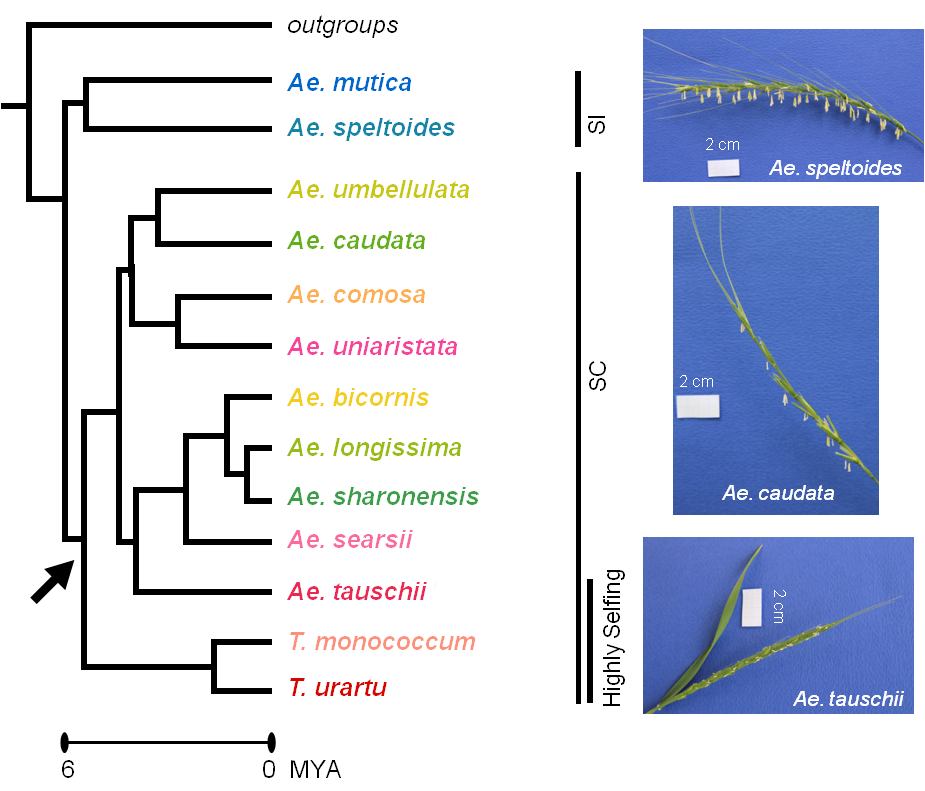
\includegraphics[width=0.60\textwidth]{./Illustrations/phylogenetic-relationships-modified.png}
    \caption{\tiny Relation phylogénétique entre les 13 espèces diploïdes du genre \textit{Aegilops} / \textit{Triticum}. Les couleurs représentent un gradient d'auto-fécondation. Les espèces heterogame (\textit{SI}) strictes sont bleues, les espèces avec un mode de reproduction mixte (\textit{SC}) sont en vert / jaune et les espèces autogame (\textit{Highly Selfing}) sont en rouge. Cette figure est issue de \cite{burgarella_mating_2024} et sa légende a été adaptée et traduite par l'auteur de ce rapport.}
    \label{fig:Phylo}
\end{figure}


% --------------------------------------------------------------- 
\end{document}
% ----------------------------  END --------------------------- 
